% !TeX root = main.tex
\section{Experiments}
\label{sec:experiments}

\subsection{Setup}
\label{sec:experiment-setup}

% Queue the double-column float before the single-column simulation floats.
\begin{table*}[!t]
    \caption{Real-robot comparison by task and execution mode. SR, success rate (\%). CS, contact stability (\%). SM, smooth rate (\%). PT, planning time (ms).}
    \label{tab:experiment-real}
    \centering
    \footnotesize
    \setlength{\tabcolsep}{0.55pt}
    \setlength{\arrayrulewidth}{0.3pt}
    \renewcommand{\arraystretch}{1.0}
    \newcommand{\taskmetrics}{\makebox[17pt]{SR} & \makebox[17pt]{CS} & \makebox[17pt]{SM} & \makebox[17pt]{PT}}
    % Replace the four entries of each task in SR, CS, SM, PT order.
    \newcommand{\taskpending}{\textendash & \textendash & \textendash & \textendash}
    \begin{tabular*}{\textwidth}{@{\extracolsep{\fill}}l@{\hspace{4pt}}l@{\hspace{3pt}}*{6}{|cccc}@{}}
        \hline
        & & \multicolumn{4}{|c|}{\shortstack{Flower\\arrangement}}
        & \multicolumn{4}{c|}{\shortstack{Plush-toy\\pickup}}
        & \multicolumn{4}{c|}{\shortstack{Cup\\stacking}}
        & \multicolumn{4}{c|}{\shortstack{Phone\\pickup}}
        & \multicolumn{4}{c|}{\shortstack{Pen pickup\\and writing}}
        & \multicolumn{4}{c@{}}{\shortstack{Pen\\spinning}} \\
        Mode & Method & \taskmetrics & \taskmetrics & \taskmetrics & \taskmetrics & \taskmetrics & \taskmetrics \\
        \hline
        Offline & \mbox{wuji-retargeting} & \taskpending & \taskpending & \taskpending & \taskpending & \taskpending & \taskpending \\
                & GeoRT            & \taskpending & \taskpending & \taskpending & \taskpending & \taskpending & \taskpending \\
                & CARD             & \taskpending & \taskpending & \taskpending & \taskpending & \taskpending & \taskpending \\
                & \mbox{CART (ours)} & \taskpending & \taskpending & \taskpending & \taskpending & \taskpending & \taskpending \\
        \hline
        Online & \mbox{wuji-retargeting} & \taskpending & \taskpending & \taskpending & \taskpending & \taskpending & \taskpending \\
                & GeoRT            & \taskpending & \taskpending & \taskpending & \taskpending & \taskpending & \taskpending \\
                & CARD             & \taskpending & \taskpending & \taskpending & \taskpending & \taskpending & \taskpending \\
                & \mbox{CART (ours)} & \taskpending & \taskpending & \taskpending & \taskpending & \taskpending & \taskpending \\
        \hline
    \end{tabular*}
\end{table*}

We compare CART with wuji-retargeting~\cite{wuji2026retargeting}, GeoRT~\cite{yin2025geort}, and CARD~\cite{dai2026card} on the Wuji2 hand. We capture demonstrations with a Moxian glove equipped with five EMF fingertip receivers and a full-palmar piezoelectric array of 460 taxels. The glove transmits synchronized EMF and tactile data at 120~Hz. CART stacks ten consecutive observation frames, from $t+1$ through $t+10$, into a sliding input window. At each update, the policy predicts a joint increment from this window and the current robot configuration $q_t$. Before capture, we tare the unloaded array to estimate its baseline and suppress noise-induced contact detections. We encode each taxel as 1 for contact or 0 for no contact when forming the policy input and scoring contact.

The Wuji2 hand lacks full-palmar tactile sensing. CARD's hardware controller uses tactile force feedback in an admittance loop over joint impedance~\cite{dai2026card}. For the CARD baseline, we replay its retargeted joint trajectories using joint impedance control. In simulation, we allow up to 5~mm of penetration between the human glove mesh and the object to approximate skin compliance.

\subsection{Simulation}
\label{sec:experiment-sim}

We replay the same demonstrations for all four methods in MuJoCo Warp (MJWarp), using the same robot, object geometry, and initial scene states. Fig.~\ref{fig:experiment-gestures} illustrates hanger and cup grasps. Table~\ref{tab:experiment-sim} lists the evaluation metrics. Fingertip RMSE measures the distance between corresponding human and robot fingertips in the aligned wrist frame. Penetration rate is the fraction of frames in which the robot hand penetrates itself or the object beyond a common tolerance. Smooth rate is the fraction of frames in which all hand-joint acceleration magnitudes stay below a shared limit. Contact retention is the fraction of demonstrated active link--frame pairs for which the corresponding robot link contacts the object. Planning time is the mean wall-clock compute time per retargeting update in milliseconds, excluding input buffering and robot execution.

\begin{table}[!t]
    \caption{Simulation comparison in MJWarp}
    \label{tab:experiment-sim}
    \centering
    \footnotesize
    \setlength{\tabcolsep}{2pt}
    \begin{tabular*}{\columnwidth}{@{\extracolsep{\fill}}lccccc@{}}
        \hline
        Method &
        \shortstack{Fingertip\\RMSE (mm)$\downarrow$} &
        \shortstack{Penetration\\(\%)$\downarrow$} &
        \shortstack{Smooth\\(\%)$\uparrow$} &
        \shortstack{Retention\\(\%)$\uparrow$} &
        \shortstack{Planning\\(ms)$\downarrow$} \\
        \hline
        wuji-retargeting & \textendash & \textendash & \textendash & \textendash & \textendash \\
        GeoRT            & \textendash & \textendash & \textendash & \textendash & \textendash \\
        CARD             & \textendash & \textendash & \textendash & \textendash & \textendash \\
        CART (ours)      & \textendash & \textendash & \textendash & \textendash & \textendash \\
        \hline
    \end{tabular*}
\end{table}

\begin{figure}[t]
    \centering
    \setlength{\tabcolsep}{2pt}
    \begin{tabular}{@{}cccc@{}}
        \scriptsize wuji-retargeting & \scriptsize GeoRT & \scriptsize CARD & \scriptsize CART \\[1pt]
        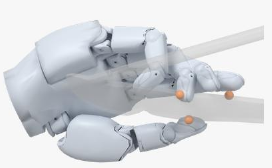
\includegraphics[width=.235\columnwidth]{figs/gesture_hanger_wuji.png} &
        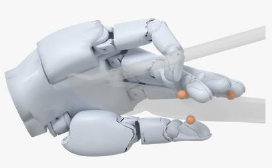
\includegraphics[width=.235\columnwidth]{figs/gesture_hanger_geort.png} &
        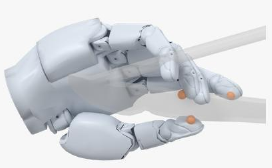
\includegraphics[width=.235\columnwidth]{figs/gesture_hanger_card.png} &
        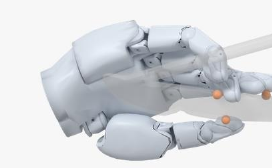
\includegraphics[width=.235\columnwidth]{figs/gesture_hanger_cart.png} \\[1pt]
        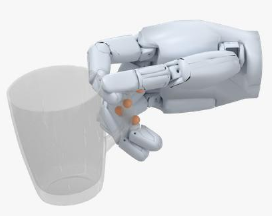
\includegraphics[width=.235\columnwidth]{figs/gesture_wuji.png} &
        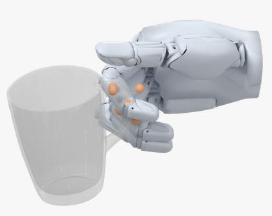
\includegraphics[width=.235\columnwidth]{figs/gesture_geort.png} &
        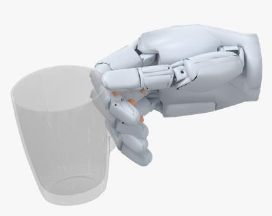
\includegraphics[width=.235\columnwidth]{figs/gesture_card.png} &
        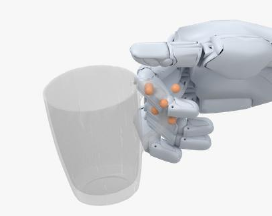
\includegraphics[width=.235\columnwidth]{figs/gesture_cart.png}
    \end{tabular}
    \caption{Example hand configurations for hanger (top) and cup (bottom) grasps. Renderings are adapted from~\cite{dai2026card}.}
    \label{fig:experiment-gestures}
\end{figure}

\emph{Draft analysis pending measurement.} We expect similar success rates for thumb-to-finger pinches across the four methods because their objectives encourage fingertip closure. For grasps with measured tactile contact, we expect wuji-retargeting and GeoRT to leave larger gaps between active taxels and the corresponding robot surfaces, especially on large objects. These gaps indicate that the robot missed contacts measured by the glove. A plausible explanation is that kinematic retargeting favors fingertip proximity in pinches and bone-direction alignment in open-hand poses. A wide grasp can therefore match the demonstrated finger directions while leaving a gap at the intended contacts. We expect CARD and CART to reduce these gaps. For continuous motion, we expect CART to require less planning time than CARD and achieve a higher smooth rate and better contact retention on the same link (Table~\ref{tab:experiment-sim}).

\subsection{Real-Robot Manipulation}
\label{sec:experiment-real}

We retarget manipulation at 1:1 physical scale with matching objects on the human and robot sides. The tasks are flower arrangement, plush-toy pickup, cup stacking, phone pickup, pen pickup and writing, and pen spinning. In the offline condition, all methods retarget the same recorded demonstrations for robot replay. In the online condition, the robot follows a live demonstration (Fig.~\ref{fig:experiment-real-frames}). For CART, the operator's observation stream leads robot-side execution by ten frames. When the robot updates from frame $t$, the synchronized EMF poses and tactile arrays through frame $t+10$ are already buffered. For each task, the operator follows a fixed gesture sequence without adapting it to the method or the robot's behavior.

Success rate is the fraction of trials in which the robot completes the entire task. Contact stability is the fraction of required link--frame contacts that the corresponding robot link maintains. The contact point may move along that link. We apply the same smooth-rate and planning-time definitions as in simulation. Table~\ref{tab:experiment-real} reports the four metrics separately for offline and online execution.

\emph{Draft analysis pending measurement.} We expect CART to achieve the highest task success rate in Table~\ref{tab:experiment-real}. We anticipate that wuji-retargeting will fail on nearly all large-object grasps, such as picking up the vase or phone, with similar failures for GeoRT. CARD's longer planning time can make online motion visibly lag, and intermittent contact loss can cause the robot to drop an object during transport after a successful pickup. We expect less visible lag with CART during live execution. This visual comparison includes buffering and robot response, whereas the reported planning time measures computation alone. We expect CART's smoother trajectories and more persistent link contact to contribute to its higher success rate.

\begin{figure*}[!t]
    \centering
    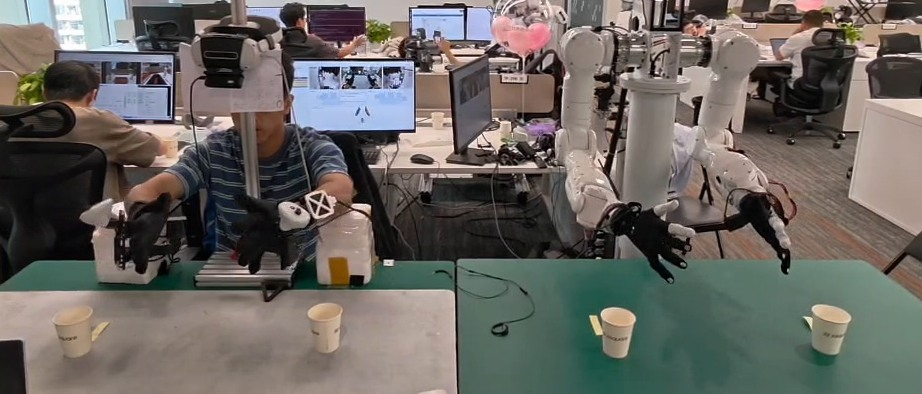
\includegraphics[width=.326\textwidth]{figs/real_robot_frame_1.jpg}\hfill
    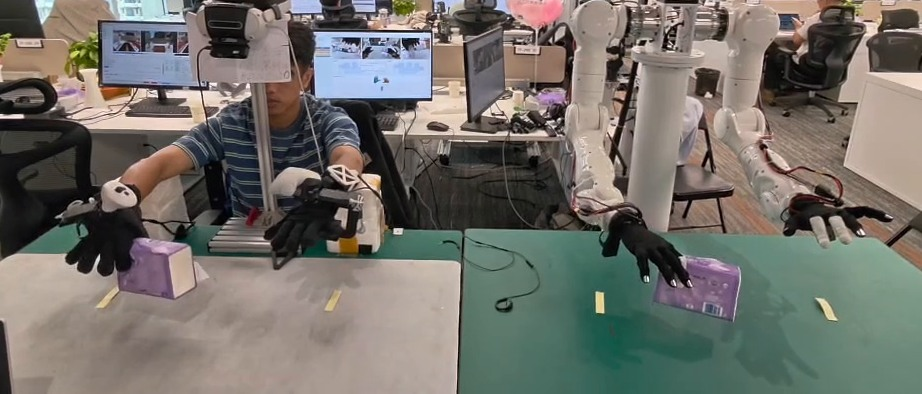
\includegraphics[width=.326\textwidth]{figs/real_robot_frame_3.jpg}\hfill
    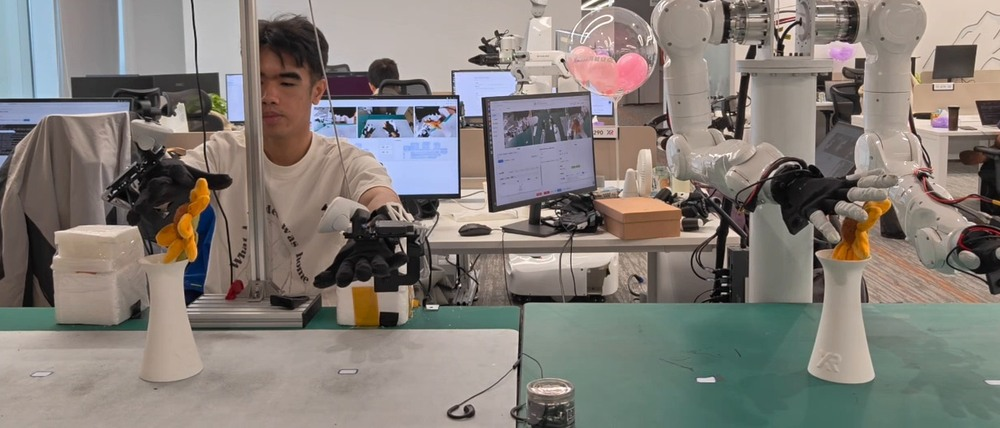
\includegraphics[width=.326\textwidth]{figs/real_robot_frame_9.jpg}\\[2pt]
    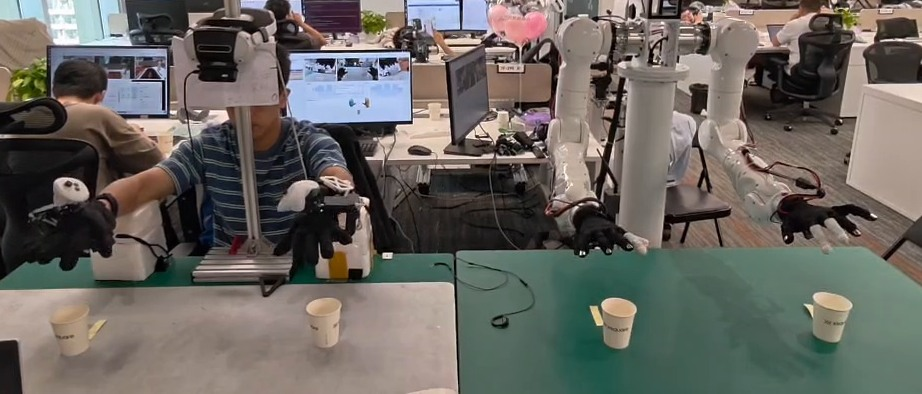
\includegraphics[width=.326\textwidth]{figs/real_robot_frame_7.jpg}\hfill
    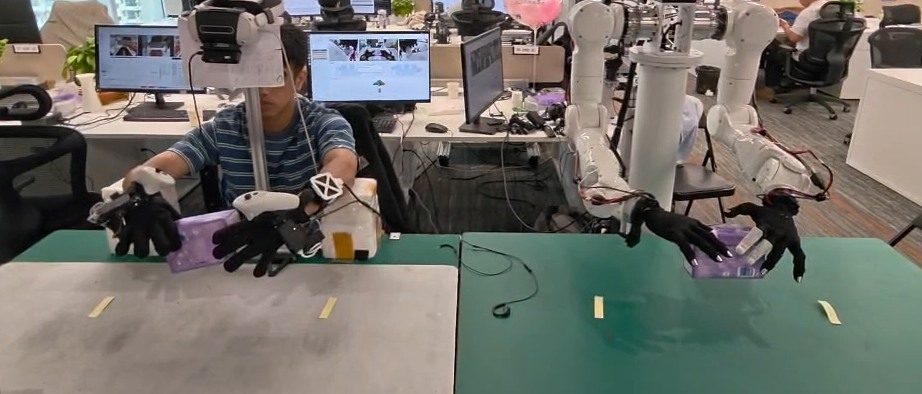
\includegraphics[width=.326\textwidth]{figs/real_robot_frame_8.jpg}\hfill
    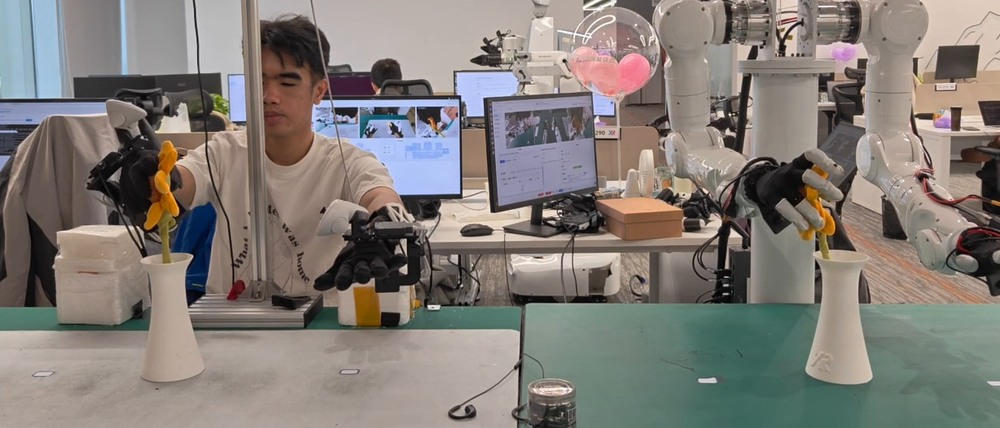
\includegraphics[width=.326\textwidth]{figs/real_robot_frame_5.jpg}\\[2pt]
    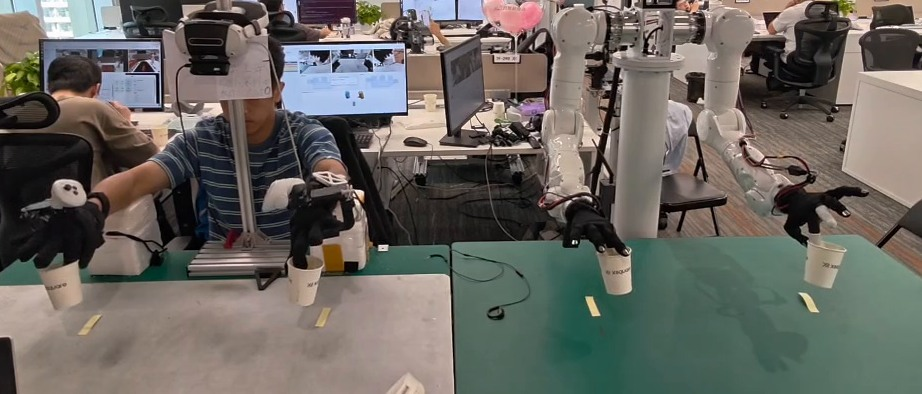
\includegraphics[width=.326\textwidth]{figs/real_robot_frame_2.jpg}\hfill
    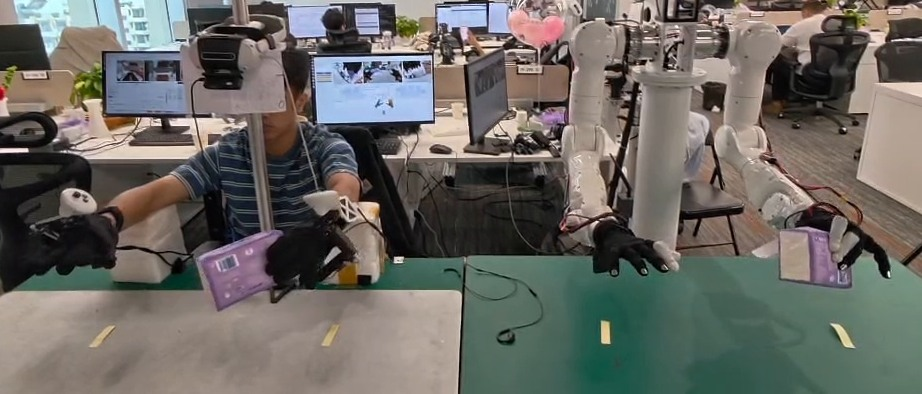
\includegraphics[width=.326\textwidth]{figs/real_robot_frame_4.jpg}\hfill
    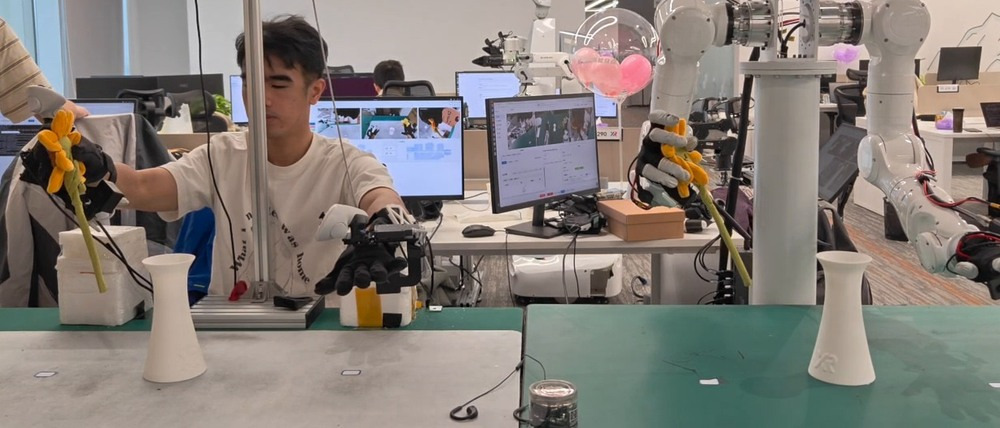
\includegraphics[width=.326\textwidth]{figs/real_robot_frame_6.jpg}
    \caption{Frames from online real-robot retargeting. Columns show cup, box, and flower handling. Rows show three stages in chronological order. The operator is on the left of each frame and the robot is on the right.}
    \label{fig:experiment-real-frames}
\end{figure*}

\subsection{Nonprehensile Manipulation}
\label{sec:experiment-nonprehensile}

We evaluate contact transfer during pen spinning, Rubik's Cube turning, and card extraction. These tasks require the fingers to release, slide, or re-establish contact as the object moves. A trial succeeds when the robot completes the prescribed pen rotation, turns the designated cube layer, or extracts the target card. We assess contact stability on the links required at each stage of the demonstration and allow the contact points to move along those links.
